\section{Introduction}

\section{Platforms}
\subsection{Amazon Mechanical Turk}
The project was introduced in 2005 and is part of the Amazon Web Services. Requesters can post tasks known as HITs (Human Intelligence Tasks) which can be solved by workers (Amazon uses another term: Turkers) 

\subsection{Crowdflower}

\section{Patterns}

\subsection{Find-Fix-Verify}
The Find-Fix-Verify pattern was introduced by the Soylent paper \cite{soylent}. The pattern divide the overall task into three stages. During the Find stage, the workers will identify patches of work done by the crowd or create new patches. For example, the workers has to select a sentence which seems to be incorrect and will need further investigations during the Fix phase. Some workers will revise the identified patches and try to provide some alternatives. The last step of the pattern will present the generated alternatives during the Fix stage to a few new workers in a randomize order. The answer with the most votes (plurality voting) will be used to replace the identified patch during the first phase. The creators of the new suggestions will be suspended so that they can't vote for their own input. To illustrate the meaning of the Find-Fix-Verify pattern, the implementation of Soylent will be discussed (Figure \ref{fixfindverify}). The approach begins by splitting a text into paragraphs. During the Find stage, the workers has to identify candidate areas for shortening in each paragraph. If a certain number of workers has selected the same area then this patch goes to the next stage. Every worker in the Fix stage has to present a shorter version of the identified patch if possible. He has also the possibility to say that the text can't be reduced. During the last step, the crowd has to select rewrites which has significant spelling, style or grammar problems or change the meaning of the sentence significantly. At the end they remove these patches by majority voting.
\begin{figure}[h!]
\centering
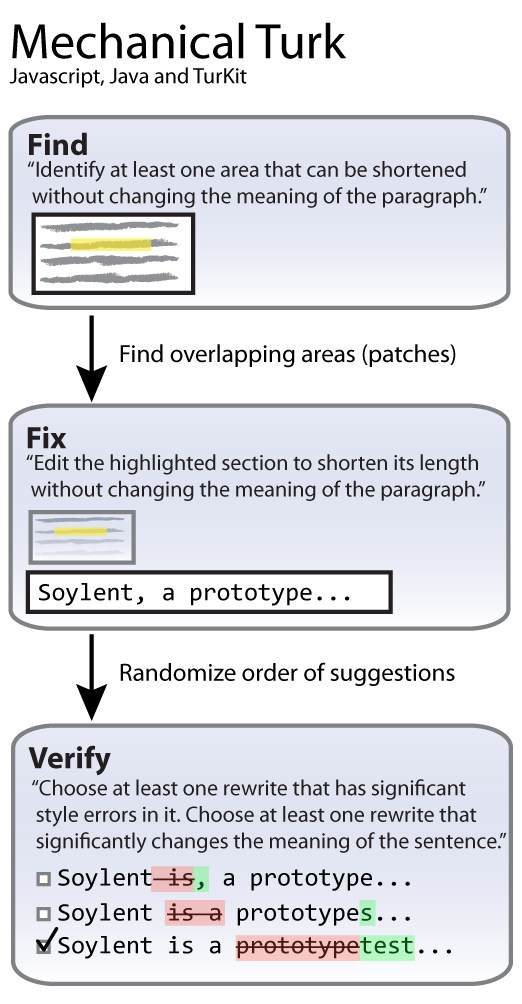
\includegraphics[scale=0.25]{images/soylent_system_overview.png}
\caption{Soylent Fix-Find-Verify pattern}
\label{fixfindverify}
\end{figure}

\subsection{Iterative}
Most of the published assignments on MTurk are independent, parallel tasks. But also iterative, sequential tasks can be useful. The authors of the TurKit paper \cite{turkit} implemented a tool which make iterative tasks possible. They developed an example application for creating an image description (Figure \ref{turkit}). During the first iteration, the worker will contribute the initial description of the provided image. The next iteration will show the initial description and a request to improve it. A few workers will evaluate the extension of the description by voting. If the extended description doesn't receive enough votes then the iteration will be ignored. The final description is generated after a fixed number of iterations. To make the iterative solution possible, the crash-an-rerun programming model was introduced by the authors of the paper. This model allows a script to be re-executed after a crash without generating costly side-effects. That means, if there is a crash during the second iteration of an iterative problem the first iteration will be skipped after re-running the script. TurKit is able to persist the state of the program and will never repeat the successfully completed task. This is helpful for prototyping algorithms.
\begin{figure}
\centering
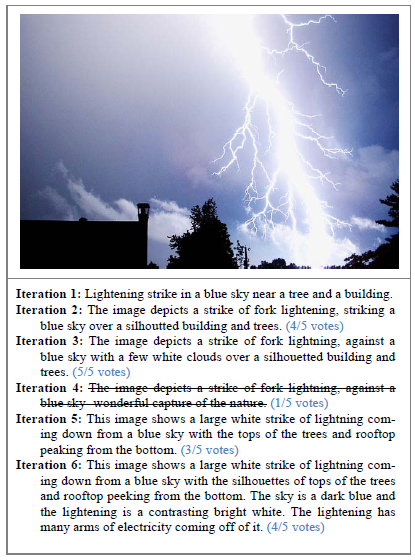
\includegraphics[scale=0.55]{images/turkit_description_example.png}
\caption{Iterative image description created by TurKit}
\label{turkit}
\end{figure}

\section{Design}
If requesters want to create new HITs then they have to consider some design guidelines\cite{crowdsourcing_tutorial}\cite{mturk_bestpractices}: 
\begin{itemize}
\item \textbf{Be as specific as possible in the instructions} If the requesters ask the workers 'Is a Ford Mustang a sports car?' is not the same as they ask 'Can a Ford Mustang accelerate from 0 to 100 km/h in 3 seconds or less?', because the second one is clearer and more precise. Sometimes it is useful to hire a technical writer for phrasing task instructions 
\item \textbf{Instructions have to be easy to read} Instructions should be split into multiple subtasks and presented as a bulleted list entries 
\item \textbf{Provide examples} The best way to present the idea of a task is to show one or multiple examples. This can help to avoid uncertainties, for example if instructions are misinterpreted or the workers have wrong expectations 
\item \textbf{Mention what won't be accepted} If a worker should write a paragraph about an  encyclopaedia article, the requester can allude in the instructions that copying contents from other website are prohibited  
\item \textbf{Tell the workers which tools they should use} 
\item \textbf{Give the workers the possibility to write down a feedback about the task} This is important to improve the design of the tasks or can help to detect spammers 
\item \textbf{Iterative and incremental development} of tasks The first draft of a task will never be perfect. With the feedbacks and results of the previous iterations, the next one will contain improvements which should avoid foregoing mistakes or design failures
\end{itemize}
MTurk best practices, Iteration, Very important, Instructions are the key

\section{Hybrid}
A lot of information systems use a hybrid crowdsourcing technology. The combination of human intelligence and machine algorithms can lead to powerful information systems which can't be realised by a pure machine approach. In most cases, the crowd is responsible to process the created content of machine algorithms or generate input data for them. 
A closer look at the CrowdSearch \cite{crowdsearch} project helps to illustrate the idea of hybrid systems. The developers implemented an image search system for cell phones. First, the system uses an automated image search to generate a set of candidate pictures. These are packed into multiple identical tasks for validation by humans and published on Amazon Mechanical Turk (Figure \ref{crowdsearch}). A simple majority voting is used to eliminating errors. After the validation of the results, the resulting image will be presented to the user. The drawbacks of such systems are that the hybrid approach generates additional costs for involving humans and the delay between publishing the tasks and receiving the corresponding results. The users of CrowdSearch can define a deadline before they query an image and the system will always return a result after the time is expired, independent if the crowd sourced tasks are completed or not. 
\begin{figure}
\centering
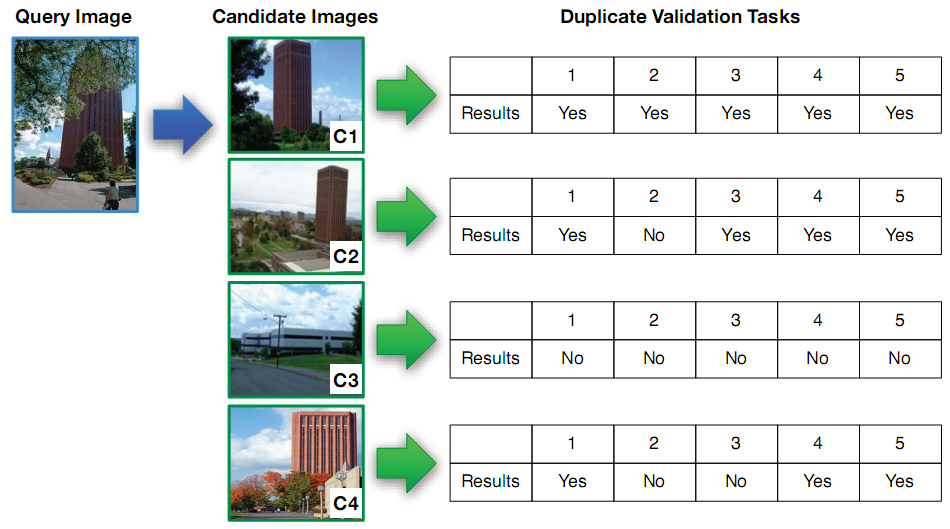
\includegraphics[scale=0.35]{images/crowdsearch_hybrid.png}
\caption{CrowdSearch hybrid image search approach}
\label{crowdsearch}
\end{figure}

\section{Quality control}
Determine the quality of completed tasks by the crowd is a very important. Workers can be lazy or are spammers which want to earn the money for free or a minimal amount of work. To evaluate the performance of a single worker, several techniques are available. 
\subsection{Majority voting }
To reduce the errors of single workers, majority voting can be used. If a majority has the same answer to a question, the requester can assume that the answer is correct. To break tie situations, a expert is necessary. 
\subsection{Honey pots }
The requesters include trap questions where they know the correct answer. If the answer of a single worker is incorrect, the requester can exclude the results or reject the task. But it's not always possible to generate honey pots. 
\subsection{Qualification test }
MTurk provides the possibility to include a qualification test at the beginning of tasks. The worker has to pass the test to have access to the real tasks and the corresponding rewards. The results of the test can be compared to an answer key automatically or by the requesters themselves. The additional effort and the determent of some workers are drawbacks of this procedure.

\section{Workflow}
A workflow is a set of tasks which are interconnected and easier to solve by crowd. The output of a single subtask will be used for one or multiple subsequent subtask. The output of the last element of the flow is the result of the entire complex task. It exists a lot of literature which covers the problematic of finding and interconnect subtask:\\

The process of decomposing complex tasks into simpler ones is not always easy and need a lot of clarifications. The developers of the Turkomatic\cite{turkomatic} tool had an obvious idea and source the workflow  decomposition out to the crowd. The workers should decide how the final workflow should look like and what are the belonging tasks. The system consists of two major parts. The meta-workflow is used to design and execute workflows by applying the price-divide-solve (PDS) procedure. The workers has to recursively divide the complex task into smaller ones until they are simple enough. After this step the workers will solve the generated tasks and other workers are asked to check the solutions. At the end, the results are combined into a cohesive answer. The second part of the Turkomatic system allows a visualisation of the created workflows and an edit function to manually adapt the crowdsourced results.\\

Another idea pursues the developers of CrowdForge\cite{crowdforge}. They designed a framework to create a workflow by using several partition, map and reduce steps. The partition step split a larger task into smaller subtasks, the map step let one or more workers process a specified task. The results of the workers are merged into a single output during the reduce step. For example, the workers should write an encyclopaedia article about a given topic (Figure \ref{crowdforgeflow}). The authors of the paper solved this problem by the presented partition/map/reduce steps. First, the partition step asks the workers to create an outline of the article by defining section headings (e.g. ''History'', ''Geography''). During the map phase, multiple workers are asked to provide a single fact about the section (e.g. ''The Empire State Building celebrated its 75th Anniversary on May 1, 2006'' if it's an encyclopaedia article about ''New York'' and the section heading is ''Attractions''). The workers has to piece the collected facts together to a completed paragraph during the reduction step.\\
The CrowdForge prototype is written in Python using the Django web framework and Boto, an interface to the Amazon Web Services which is available in Python. The user can define complex flows by creating HIT templates (which can be either a partition, map or reduce task) and dependencies between the templates to define a flow. Flows are implemented as Python classes. The prototype is also responsible for the sequential coordination between the HITs (including data transfer). Multiple independent flows can be executed simultaneously. One of the limitations is that CrowdForge does not support iteration or recursion. The further development of the project was suspended in 2011.
\begin{figure}
\centering
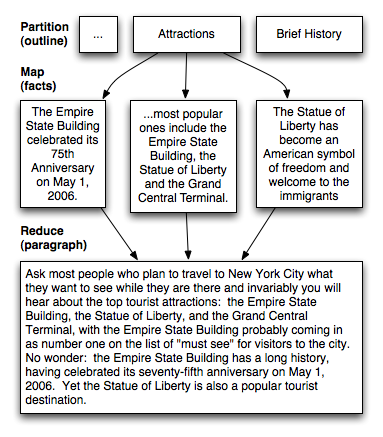
\includegraphics[scale=0.5]{images/crowdforge-article.png}
\caption{CrowdForge example workflow}
\label{crowdforgeflow}
\end{figure}

The same crew developed CrowdWeaver\cite{crowdweaver} which is an advancement of the CrowdForge project. They use CrowdFlower, an other crowdsourcing platform, instead of Amazon Mechanical Turk. On CrowdFlower, the requester can create tasks on multiple markets (including MTurk). Flows can be created visually and doesn't assume any programming skills. Another feature is the tracking and notification of crowd factors, for example latency or price.

Jabberwocky

\section{Incentives}

\subsection{Game}
The ESP game\cite{esp} makes the labelling of any kind of images on the web possible. There are no guidelines to provide images and no computer vision method exists which can handle the diversity of all images. Search engines are dependent on accurate image descriptions to represent relevant results. Therefore, another approach was introduced by the article. A online, web-based game was developed to attract workers. Two players are randomly assigned to label the same image simultaneously. There is no possibility to communicate with the game partner. Now, every player has to guess the description of the image independently without using the 'Taboo words'. These words are evaluated by a prior round and will be ignored for the actual turn. If there is a match between both players, the score will be increased and another image description was detected. The discovered word will only be taken as a valid description and 'Taboo word' if a predefined number of players had the same agreement.  The duration of the whole game is 150 seconds and both parties can guess as many images as possible within this time. 
During a period of four months, the game was played by 13'630 people and 1'271'451 labels for 293'760 images were generated. These numbers show the power of the idea. The players (crowd) didn't know what's going on behind the scenes and they also didn't realise the purpose of their inputs.

Money, Financial Incentives and the ''Performance of Crowds''

